
\chapter{Classificação de vulnerabilidades}
\label{chap:classificacao}

	A classificação de vulnerabilidades representa enorme desafio.
	Nos dias de hoje, não existe nenhum padrão aceito globalmente para essa tarefa.
	Ainda assim, já houve vários avanços na área. 
	Existem padrões para enumerar e catalogar vulnerabilidades, bem como propostas
	que podem criar bases para uma classificação que venha a ser aceita pela comunidade.
	Métricas, relativas	à gravidade e ao impacto, também estão disponíveis
	e são empregadas no auxílio às instituições nas tomadas	de decisões.

	
	No trabalho de Seacord e Householder, \cite{Seacord2005}, temos os fatores que motivam a
	busca pela organização das vulnerabilidades em classes:
	\begin{itemize}
		\item{O entendimento das ameaças que elas representam.}
		\item{Correlacionamento de incidentes, de \textsl{exploits} e de artefatos.}
		\item{Avaliação da efetividade das ações de defesa.}
		\item{Descoberta de tendências de vulnerabilidades.}
	\end{itemize}

	
	Vemos, portanto, que a taxonomia\footnote{Ciência da classificação.} das vulnerabilidades
	pode trazer uma série de benefícios para seu entendimento, tratamento e prevenção.
	Nesse capítulo, nosso intuito é abordar a dificuldade nesse processo e apresentar
	os avanços já obtidos nesse sentido.  


	\section{A dificuldade em classificar; estágio já alcançado: enumeração}
		Antes de entrarmos no mérito das vulnerabilidades, é preciso definir
		com precisão dois termos que utilizaremos por todo o capítulo: classificar e enumerar.
		Como veremos, a taxonomia é mais custosa que a enumeração.

		\subsection{Classificar}
			\label{subsec:classificar}
			Como podemos encontrar em \cite{Holanda1975}, classificar implica "distribuir em classes e/ou grupos
			segundo um sistema". Logo, para a classificação, é preciso haver uma metodologia que possa
			separar os itens em estudo em diferentes grupos. A ciência que estuda esse processo
			é chamada taxonomia. Ela é guiada, conforme \cite{Gregio2005_1}, pelos princípios taxonômicos.
			São eles:
			\begin{description}
				\item[Exclusão mútua]
					Um item não podem ser categorizado simultaneamente em dois grupos.
				\item[Exaustividade]
					Os grupos, unidos, incluem todas as possibilidades.
				\item[Repetibilidade]
					Diferentes pessoas extraindo a mesma característica do objeto devem concordar com
					o valor observado.
				\item[Aceitabilidade]
					Os critérios devem ser lógicos e intuitivos para serem aceitos pela comunidade.
				\item[Utilidade]
					A classificação pode ser utilizada na obtenção de conhecimento na área de pesquisa.
			\end{description}

			
			Vemos que os critérios para a taxonomia são exigentes e pressupõem uma metodologia
			cuidadosamente gerada para atendê-los. 

		\subsection{Enumerar}
			A enumeração é um processo semelhante a 
			"indicar por números; relacionar metodicamente"; como encontramos
			em \cite{Holanda1975}.
			Trata-se, portanto, de algo muito mais simples que a classificação.
			Mesmo sendo mais simples, é extremamente importante pois permite
			que os itens enumerados sejam facilmente apontados e diferenciados entre si.
			
			
			Sem um procedimento de enumeração dos objetos de estudo, adotado de comum acordo,
			não é possível que duas partes se comuniquem sem risco de cometerem enganos. 
			Quem garante que estão tratando exatamente da mesma coisa naquele momento?
			Logo a enumeração é essencial para o devido entendimento sobre os objetos
			de estudo.

		\subsection{Da enumeração à classificação}
			No trabalho de Mann, \cite{Mann1999}, há um excelente paralelo entre a
			questão abordada nesse capítulo e o advento da tabela 
			periódica\footnote{Dispõe sistematicamente os elementos de acordo com suas propriedades permitindo
			uma análise multidimensional.} na Química. 
			A organização dos elementos da forma como conhecemos hoje na tabela periódica
			foi um processo longo que culminou com as ideias de Dimitri Mendeleev.
			Outros químicos que o precederam foram responsáveis pela identificação e
			listagem dos elementos. Isso possibilitou um melhor estudo e uma maior
			troca de informação precisa entre os pesquisadores.


			Segundo Mann, a tabela periódica só pode ser efetivamente criada graças
			aos esforços daqueles que enumeraram os elementos de forma mais simples
			antes de Mendeleev. O trabalho deles permitiu a interoperabilidade
			necessária para o surgimento da tabela periódica.
			Da mesma forma, nos anos antecedentes a 2000, a comunidade que estudava
			e acompanhava as vulnerabilidades estava num patamar semelhante àqueles
			que precederam Mendeleev. Ou seja, sequer havia uma enumeração mais
			amplamente aceita e reconhecida das vulnerabilidades que permitisse
			avanços suficientes para uma taxonomia.

			
			Citamos o ano de 2000 como parâmetro, pois nessa época, 1999, surgiria um projeto
			que se tornaria referência para a criação de uma padronização da enumeração
			de vulnerabilidades. Não seria ainda um evento comparável à criação da
			tabela periódica para Química (pois não trouxe a taxonomia) 
			mas certamente lançaria as bases para
			a interoperabilidade exigida para estudos mais aprofundados na área.
			Estamos falando da criação do 
			CVE(Common Vulnerabilities and Exposures)\footnote{http://cve.mitre.org}\footnote{Na época
			de sua criação era originalmente conhecido por Common Vulnerabilities Enumeration - vide
			\cite{Meunier2006} pg. 9.}
			pelo MITRE. A seção \ref{sec:cve} traz mais detalhes.


			Podemos dizer, portanto, que atualmente, embora não tenhamos uma taxonomia
			amplamente aceita pela comunidade, já foi atingido o estágio de enumeração.
			Projetos como o CVE podem ser considerados como marcos dessa etapa.
			A seguir, iremos abordar em mais detalhes o surgimento e o funcionamento dele.
			Isso nos possibilitará compreender melhor a complexidade da classificação
			das vulnerabilidades bem como irá facilitar o entendimento dos capítulos
			seguintes que abordam \textsl{exploits}.
			

	\section{CVE}
	\label{sec:cve}

		\subsection{Surgimento e objetivos}
			Para deixar mais nítida a dificuldade de interoperabilidade
			das organizações no que se refere a ameaças de segurança na época
			que antecede o CVE, segue abaixo uma tabela, extraída de \cite{Martin2001}.
			A tabela \ref{tab:torre_babel}, mostra
			como diferentes organizações se referiam à mesma vulnerabilidade
			em 1998. Trata-se de um verdadeira Torre de Babel.

			\begin{table}
				\begin{tabular}{|l|c|c|c|c|}
					\hline
						\textbf{Organização} & \textbf{Como se referia à vulnerabilidade}\\
					\hline
						CERT\footnotemark[1] & CA-96.06.cgi\_example\_code\\
					\hline
						Cisco Systems\footnotemark[2] & http - cgi-phf\\
					\hline
						DARPA & 0x00000025 = http PHF attack\\	
					\hline
						IBM ERS & ERS-SVA-E01-1996:002.1\\	
					\hline
						Security Focus\footnotemark[3] & \#629 - phf Remote Command Execution Vulnerability\\	
					\hline
				\end{tabular}
				\footnotetext[1]{site}
				\footnotetext[2]{site}
				\footnotetext[3]{site}
				\caption{Uma vulnerabilidade: diversos nomes e nenhum entendimento}\label{tab:torre_babel}
			\end{table}
			

			O CVE, como dito anteriormente, surge em 1999 e seu maior objetivo, como podemos
			ler em sua FAQ, \cite{CVE2010}, é tornar mais fácil
			o compartilhamento de informações sobre vulnerabilidades utilizando uma enumeração comum.
			Essa enumeração é realizada através da manutenção de uma lista na qual, conforme
			encontramos em \cite{Santos2004}, valem os seguintes princípios:
			\begin{itemize}
				\item{Atribuição de um nome padronizado e único a cada vulnerabilidade.}
				\item{Independência das diferentes perspectivas em que a vulnerabilidade ocorre.}
				\item{Abertura total voltada ao compartilhamento pleno das informações.}
			\end{itemize}


			Segundo a própria organização, vide \cite{CVE2010}, o CVE não possui um objetivo 
			inicial de conter alguma espécie de taxonomia. Essa é considerada uma área de pesquisa
			ainda em desenvolvimento. É esperado que, com o auxílio prestado pela
			catalogação das vulnerabilidades já constitua um importante passo para que
			isso ocorra.

			\begin{figure}
				\begin{center}
					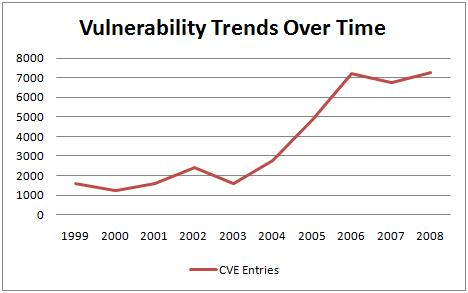
\includegraphics[width=0.65\textwidth]{vulnerabilidades_CVE.jpg}
					\caption{Vulnerabilidades registradas no CVE ao longo do tempo - retirada 
							de \cite{Florian2009}}
					\label{fig:vulnerabilidades_CVE}
				\end{center}
			\end{figure}

			
			Na figura \ref{fig:vulnerabilidades_CVE}, podemos visualizar um histórico
			da quantidade de vulnerabilidades adicionadas. Nos últimos anos podemos
			perceber que os incidentes registrados ficam na média de 7000.
			Isso mostra relevância que o projeto do CVE alcançou.
			
			 
		
		\subsection{Funcionamento}
			O CVE é formado por uma junta de especialistas em segurança dos meios acadêmico, comercial e
			governamental. Eles são responsáveis por analisar e definir o que será feito dos reports passados
			pela comunidade - se eles devem ou não se integrar àqueles já pertencentes à lista.
			Cabe a eles definir nome, descrição e referências para cada nova ameaça.


			Esse processo inicia quando uma vulnerabilidade é reportada.
			Ela assume um CAN(Candidate Number), número de candidata.
			Até que ela seja adicionada à lista, ele permanece com um CAN que
			a identificará. Apenas após o devido estudo e aprovação do caso pela junta
			responsável, é que ela assume um identificador CVE.

			
			Os identificadores CVE são definidos conforme o padrão: CVE-2010-0021.
			Onde, separados por '-', há 3 partes. A primeira é fixa: CVE.
			A segunda refere-se ao ano de surgimento; enquanto a terceira
			indica o número sequencial daquela vulnerabilidade entre todas
			aquelas que foram adicionadas naquele ano. Logo, no exemplo fornecido,
			essa seria a vigésima primeira de 2010.
		
			
			Uma vez integrada, a vulnerabilidade passa a estar publicamente disponível.
			Essa abertura pode servir de auxílio aos atacantes - pois informações
			sobre possíveis furos de segurança são sempre bem vindas a eles.
			Porém, conforme podemos verificar na FAQ do CVE, \cite{CVE2010}, há uma série
			de motivos pelos quais a disponibilidade desses dados supera o risco
			oferecido pela exposição. São eles:
			\begin{itemize}
				\item{O CVE está restrito a publicar vulnerabilidades já conhecidas.}
				\item{Por diversas razões, a comunidade de segurança de informação
					sofre mais para compartilhar dados sobre as ameças
					que os atacantes.}
				\item{É muito mais custo a uma organização proteger toda sua rede
					contra as ameças que a um atacante descobrir e explorar uma delas para
					comprometer alguma das redes.}
			\end{itemize}
			
			

		
		
		
	\section{Propostas taxonômicas}
		Como foi referenciado anteriormente, não há padrão amplamente aceito
		para a taxonomia de vulnerabilidades.
		Mesmo assim, há diversas propostas que buscam resolver essa questão em aberto.
		
		
		O trabalho de \cite{Gregio2005} faz um levantamento amplo de algumas
		dessas alternativas. Mas, como veremos, nenhuma delas atinge os objetivos
		de uma taxonomia plena - apresentados na seção \ref{subsec:classificar}.
		Assim, buscaremos discutir as ideias para as metodologias
		de classificação com o intuito de apontar suas vantagens e fraquezas.

	\section{Métricas para vulnerabilidades}
		Comparar objetivamente vulnerabilidades de acordo com sua criticidade é
		algo muito útil para as organizações.
		Isso possibilita que os gestores mensurem o grau de urgência com que devem
		ser tratadas as ameaças. Podemos considerar esse procedimento
		como um tipo rudimentar de classificação.

		
		Para essa finalidade existe uma alternativa relativamente recente, o CVSS
		(Common Vulnerability Scoring System), criado em 2005.

		\subsection{CVSS}
			O CVSS é um \textsl{framework} aberto para atribuição de escore a vulnerabilidades.
			
			Explicar objetivos.

			Apresentar breve histórico.

			Mostrar os critérios usados.
			
			Como calcular.

			Exemplos.

			Quem já utiliza o CVSS (como a Oracle).
		\begin{figure}
			\begin{center}
				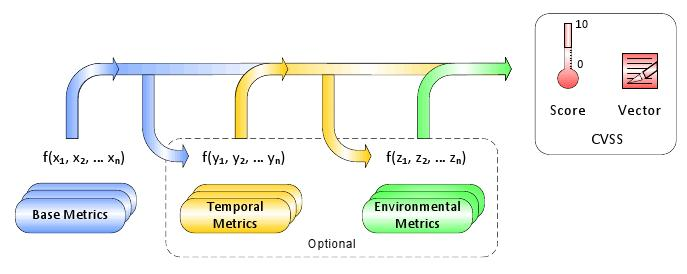
\includegraphics[width=0.85\textwidth]{cvss_metricas_equacoes.jpg}
				\caption{Aplicação das métricas e equações do CVSS - Fonte: \cite{Mell2007}}
				\label{fig:cvss_metricas_equacoes}
			\end{center}
		\end{figure}

			

